% chktex-file 1
% chktex-file 8
% chktex-file 13
% chktex-file 24
% chktex-file 36
% chktex-file 44

\chapter{Performanzanalyse}

\section{Qualität}

Im Folgenden wird die Qualität der erstellten Diagramme untersucht.

Zunächst soll analysiert werden, welche KI-Modelle besonders hochwertige Diagramme erzeugen können. 
Aspekte wie Zeitaufwand und Kosten werden in diesem Abschnitt bewusst nicht berücksichtigt, da der 
Fokus ausschließlich auf der Ergebnisqualität liegt.

Für die Untersuchung werden mit verschiedenen KI-Modellen Diagramme generiert. 
Dabei kommt eine einheitliche Prozessbeschreibung (siehe Prompt~\ref{prompt:quality-1}) zum Einsatz. 
Diese wurde bewusst nicht einfach oder kurz gehalten, sondern möglichst komplex formuliert, 
um zu evaluieren, welche Modelle in der Lage sind, anspruchsvolle und detaillierte Beschreibungen 
korrekt zu verarbeiten und umzusetzen.

In einem weiteren Schritt wird auch ein vereinfachter Prompt verwendet. 
Ziel ist es zu überprüfen, ob einzelne Modelle selbst bei weniger komplexen Prozessbeschreibungen 
Schwierigkeiten aufweisen und somit grundlegende Anforderungen nicht zuverlässig erfüllen können.

\subsection{Modellunterschiede komplexer Diagramme}

Welches KI Modell kann besonders gut aus komplexen Prozessbeschreinungen BPMN Diagramme erstellen?

Hierfür werden einige der aktuellsten Modelle der implentierten Anbieter getestet und die 
Ergebnisse verglichen.
Gleichzeitig wird zudem auch zwischen den verwendeten Formaten XML und JSON, welche auf 
Seite~\pageref{sec:format} beschrieben sind, unterschieden.
Die Modelle, welche getestet werden sind:
\begin{itemize}
    \item \textbf{Gemini 2.5 Pro} 
        erzeugt Diagramm~\ref{fig:gemini-2-5-pro-json} in JSON 
        und Diagramm~\ref{fig:gemini-2-5-pro-xml} in XML
    \item \textbf{Gemini 2.5 Flash} 
        erzeugt Diagramm~\ref{fig:gemini-2-5-flash-json} in JSON 
        und Diagramm~\ref{fig:gemini-2-5-flash-xml} in XML
    \item \textbf{ChatGPT 5.2} 
        erzeugt Diagramm~\ref{fig:gpt-5-2-json} in JSON 
        und Diagramm~\ref{fig:gpt-5-2-xml} in XML
    \item \textbf{ChatGPT 5.1} 
        erzeugt Diagramm~\ref{fig:gpt-5-1-json} in JSON 
        und Diagramm~\ref{fig:gpt-5-1-xml} in XML
    \item \textbf{ChatGPT 4.1} 
        erzeugt Diagramm~\ref{fig:gpt-4-1-json} in JSON 
        und Diagramm~\ref{fig:gpt-4-1-xml} in XML
    \item \textbf{Grok 4}
        erzeugt Diagramm~\ref{fig:grok-4-json} in JSON 
        und Diagramm~\ref{fig:grok-4-xml} in XML
    \item \textbf{Grok 4.1 Fast}
        erzeugt Diagramm~\ref{fig:grok-4-1-json} in JSON 
        und Diagramm~\ref{fig:grok-4-1-xml} in XML
    \item \textbf{Claude Opus 4.5} 
        erzeugt Diagramm~\ref{fig:claude-opus-4-5-json} in JSON 
    \item \textbf{Claude Sonnet 4.5} 
        erzeugt Diagramm~\ref{fig:claude-sonnet-4-5-json} in JSON
\end{itemize}
Es wird für alle die einheitliche Prozessbeschreibung~\ref{prompt:quality-1} verwendet.
Um auch zu testen, ob die Modelle in der Lage sind, die gewünschte Ausgabesprache anhand der Eingabesprache 
zu erkennen und zu verwenden,
wird diese Prozessbeschreibung in deutsch geschrieben.

\begin{prompt}[H]
    \noindent\fbox{
      \parbox{.96\textwidth}{
        Der Kunde sendet online seine Bestellung an die E-Commerce-Plattform.
        Dort wird parallel in der Finanzbuchhaltung die Zahlungsautorisierung angefragt, wobei eine Kreditprüfung (automatisch, manuell nur über 200€) erfolgt.
        Die Finanzbuchhaltung meldet dann „Zahlung OK“ oder „abgelehnt“ zurück, wobei nach einer Stunde ohne Antwort eine Erinnerung folgt.
        Gleichzeitig verzweigt der Prozess: Es wird für jeden Artikel der Bestand beim Lager \& Logistik angefragt, und wenn ein Artikel eine Sonderanfertigung ist, 
        geht zusätzlich eine Anfrage an die Fertigung. Im Lager wird bei Verfügbarkeit reserviert, bei Nichtverfügbarkeit der Kunde informiert und eine Nachbestellung ausgelöst.
        Die Fertigung beginnt den Subprozess der Sonderanfertigung und sendet nach Abschluss eine Fertigstellungsnachricht an die Plattform und eine Abholbereitmeldung ans Lager.
        Die E-Commerce Plattform wartet auf alle Rückmeldungen. Bei Zahlungsablehnung wird alles storniert und der Kunde benachrichtigt.
        Bei Erfüllung geht der Kommissionierungsauftrag ans Lager (mit Eskalation an den Manager nach 48 Stunden).
        Das Lager kommissioniert, verpackt und sendet den Lieferschein an die Finanzbuchhaltung sowie eine Abholanforderung an den Versanddienstleister.
      }
    }
    \caption{Komplexe Prozessbeschreibung für einen Qualitätstest}
    \label{prompt:quality-1}
\end{prompt}

Vorab ist es nun wichtig zu erwähnen, dass mit diesem Prompt kein Diagramm von
\texttt{Claude Opus 4.5} mit XML erstellt werden konnte, da dies die 
Maximaltokenanzahl dieses Modells übersteigt.

\paragraph{Formale Richtigkeit} \label{sec:correctness-formal}
Damit wird geprüft, ob das Diagramm regelkonform nach BPMN 2.0 ist.
Hierbei ist entscheidend, wie viele formatbedingte und konventionelle Fehler in 
dem Diagramm erzeugt werden.
Dazu zählen unter anderem:

\begin{itemize}
    \item Jeder Flow beginnt mit einem Start Event und endet mit einem End Event.
    \item Gateways haben korrekte Ein- und Ausgänge (z. B. XOR, AND, Event-Based).
    \item Kein Element hat ungültige Sequenzen (z. B. Aktivitäten direkt nach Nachrichtenflüssen).
    \item Es gibt keine ID Duplikate.
    \item Keine grundlegenden Formatfehler.
    \item Alle Referenzen sind richtig.
\end{itemize}

Bei dem Test wurden alle Fehler gesammelt und zusammengefasst.
Die Fehler wurden mit Hilfe von bpmn-moddle
\footnote{\url{https://github.com/bpmn-io/bpmn-moddle}} gesammelt.
Hierbei ist ein Fehler, durch den das gesamte Diagramm nicht angezeigt werden kann,
ein kritischer Fehler. Tritt ein kritischer Fehler auf, wird die Generierung wiederholt, 
bis keine kritischen Fehler erstellt werden.
Ein Fehler, durch den ein einzelnes Element
nicht angezeigt werden kann, ist ein elementarer Fehler.
Bei diesem Test wurde auf das vorgestellte Schema Constraining auf Seite~\pageref{sec:schema}
verzichtet, um den Modellen möglichst viel Freiraum zu geben und dadurch die Richtigkeit der 
Diagramme besser beurteilen zu können.
Das jeweils ohne kritische Fehler erstellte Diagramm der Modelle wird in den Abbildungen:
~\ref{fig:gemini-2-5-pro-json},
~\ref{fig:gemini-2-5-pro-xml},
~\ref{fig:gemini-2-5-flash-json},
~\ref{fig:gemini-2-5-flash-xml},
~\ref{fig:gpt-5-1-json},
~\ref{fig:gpt-5-1-xml},
~\ref{fig:gpt-5-2-json},
~\ref{fig:gpt-5-2-xml},
~\ref{fig:gpt-4-1-json},
~\ref{fig:gpt-4-1-xml},
~\ref{fig:grok-4-json},
~\ref{fig:grok-4-xml},
~\ref{fig:grok-4-1-json},
~\ref{fig:grok-4-1-xml},
~\ref{fig:claude-sonnet-4-5-json}
und~\ref{fig:claude-opus-4-5-json} dargestellt.
Die Anzahl an Fehlern ist in Tabelle~\ref{tab:qualitat-formal} zu sehen.

\begin{table}[hbt]
  \centering
  \renewcommand{\arraystretch}{1.2}
  \begin{tabular}{|l|l|c|c|}
    \hline
    \multicolumn{2}{|l|}{\textbf{Modell}} & \textbf{kritische Fehler} & \textbf{elementare Fehler} \\ \hline
    \multirow{2}{*}{\textbf{Gemini 2.5 Pro}}    & JSON & 0 & 0   \\ 
                                                & XML  & 1 & 0   \\ \hline
    \multirow{2}{*}{\textbf{Gemini 2.5 Flash}}  & JSON & 0 & 33  \\ 
                                                & XML  & 0 & 24  \\ \hline
    \multirow{2}{*}{\textbf{ChatGPT 5.2}}       & JSON & 0 & 4   \\ 
                                                & XML  & 2 & 0   \\ \hline
    \multirow{2}{*}{\textbf{ChatGPT 5.1}}       & JSON & 0 & 0   \\ 
                                                & XML  & 0 & 2   \\ \hline
    \multirow{2}{*}{\textbf{ChatGPT 4.1}}       & JSON & 0 & 13  \\ 
                                                & XML  & 0 & 5   \\ \hline
    \multirow{2}{*}{\textbf{Grok 4}}            & JSON & 0 & 16  \\ 
                                                & XML  & 0 & 0   \\ \hline
    \multirow{2}{*}{\textbf{Grok 4.1 Fast}}     & JSON & 0 & 20  \\ 
                                                & XML  & 0 & 3   \\ \hline
    \textbf{Claude Opus 4.5}                    & JSON & 0 & 0   \\ \hline
    \textbf{Claude Sonnet 4.5}                  & JSON & 0 & 26  \\ \hline
  \end{tabular}
  \caption{Formale Richtigkeit}
  \label{tab:qualitat-formal}
\end{table}

Die Auswertung der formalen Richtigkeit zeigt, dass sich deutliche Leistungsunterschiede 
erkennen lassen. 

Claude Opus 4.5, Gemini 2.5 Pro und ChatGPT 5.1 stechen insbesondere im JSON Format hervor, 
da hier keine formalen Fehler festgestellt wurden. 
Die erzeugten Diagramme halten die grundlegenden BPMN-2.0-Konventionen ein. 
Damit zeigen diese Modelle eine hohe Eignung für die Modellierung komplexer Prozesse. 

Im XML-Format offenbaren sich auch stärkere Unterschiede. 
Während einige Modelle, darunter Gemini 2.5 Pro und ChatGPT 5.2, kritische Fehler erzeugen, 
die eine erneute Generierung erforderlich machen, liefert Grok 4 in diesem Format formal 
fehlerfreie Ergebnisse. 
Dies deutet darauf hin, dass Grok 4 besonders gut mit der strengen Struktur und den 
Referenzabhängigkeiten von BPMN-XML umgehen kann und sich daher besonders für Diamgrammerstellungen
ohne Zwischenformat eignet.
Interessant ist auch, dass, obwohl Gemini 2.5 Pro und ChatGPT 5.2 kritische Fehler erstellen,
sie bei einer nicht-kritischen Erstellung eines Diagramms auch keine elementaren Fehler erstellen.

\paragraph{Semantische Richtigkeit} \label{sec:correctness-semantic}
Hier geht es darum, ob das Modell inhaltlich korrekt ist.
Dazu werden folgende Aspekte überprüft:

\begin{itemize}
    \item Bildet das Diagramm den beschriebenen Prozess korrekt ab?
    \item Sind alle nötigen Komponenten vorhanden?
    \item Wurden unnötige Komponenten hinzugefügt?
    \item Stimmen Reihenfolgen und Abhängigkeiten überein?
\end{itemize}

In der folgenden Tabelle~\ref{tab:qualitat-semantisch} wurde untersucht, wie viele
Komponenten in den einzelnen Diagrammen jeweils fehlen bzw.\ ungewünscht 
hinzugefügt wurden.

\begin{table}[hbt]
    \centering
    \renewcommand{\arraystretch}{1.2}
    \begin{tabular}{|l|l|c|c|}
      \hline
      \multicolumn{2}{|l|}{\textbf{Modell}} & \textbf{fehlend} & \textbf{unnötig} \\ \hline
      \multirow{2}{*}{\textbf{Gemini 2.5 Pro}}    & JSON & 0 & 4   \\ 
                                                  & XML  & 1 & 0   \\ \hline
      \multirow{2}{*}{\textbf{Gemini 2.5 Flash}}  & JSON & 10& 6   \\        
                                                  & XML  & 0 & 4   \\ \hline
      \multirow{2}{*}{\textbf{ChatGPT 5.2}}       & JSON & 1 & 8   \\ 
                                                  & XML  & 1 & 2   \\ \hline
      \multirow{2}{*}{\textbf{ChatGPT 5.1}}       & JSON & 9 & 2   \\ 
                                                  & XML  & 7 & 8   \\ \hline
      \multirow{2}{*}{\textbf{ChatGPT 4.1}}       & JSON & 15& 2   \\ 
                                                  & XML  & 40& 1   \\ \hline
      \multirow{2}{*}{\textbf{Grok 4}}            & JSON & 8 & 0   \\ 
                                                  & XML  & 3 & 0   \\ \hline
      \multirow{2}{*}{\textbf{Grok 4.1 Fast}}     & JSON & 5 & 3   \\ 
                                                  & XML  & 2 & 1   \\ \hline
      \textbf{Claude Opus 4.5}                    & JSON & 0 & 4   \\ \hline
      \textbf{Claude Sonnet 4.5}                  & JSON & 11& 1   \\ \hline 
    \end{tabular}
    \caption{Semantische Richtigkeit}
    \label{tab:qualitat-semantisch}
\end{table}

Die Ergebnisse in Tabelle~\ref{tab:qualitat-semantisch} zeigen, dass die Modelle deutliche Unterschiede 
hinsichtlich der Vollständigkeit der erzeugten Diagramme aufweisen. 

Besonders positiv fällt erneut Claude Opus 4.5 auf, welcher im JSON-Format keine fehlenden Komponenten erzeugt. 
Zwar wurden einige zusätzliche, nicht explizit geforderte Elemente ergänzt, diese beeinflussen jedoch die 
grundlegende Prozesslogik nicht wesentlich. 
Insgesamt deutet dieses Ergebnis auf ein sehr gutes semantisches Prozessverständnis hin.

Gemini 2.5 Pro zeigt ebenfalls eine hohe semantische Qualität. 
Im JSON-Format fehlen keine Prozessbestandteile, allerdings wurden mehrere unnötige Komponenten ergänzt. 
Im XML-Format fehlt nur ein einziges Element, dafür wurde kein einziges unnötiges hinzugefügt.
Dies legt nahe, dass das Modell den Prozess grundsätzlich korrekt interpretiert.

Die Modelle der ChatGPT-Reihe liefern insgesamt gemischte Ergebnisse. 
Während ChatGPT 5.2 im Vergleich zu älteren Versionen deutlich weniger fehlende Komponenten aufweist, 
insbesondere im XML-Format, tendiert es dazu, zusätzliche Tasks zu ergänzen, 
die nicht explizit in der Prozessbeschreibung stehen. 
ChatGPT 5.1 und insbesondere ChatGPT 4.1 zeigen hingegen eine deutlich höhere Anzahl fehlender 
Komponenten.

Grok 4 und Grok 4.1 Fast positionieren sich im Mittelfeld. 
Beide Modelle erfassen den Kernprozess weitgehend korrekt und verzichten nahezu vollständig auf 
unnötige Ergänzungen. 

Abgesehen von den ausgearbeiteten Komponentenfehlern lassen sich noch einige weitere Eigenheiten erkennen.
Bei Claude Sonnet 4.5 und Gemini 2.5 Flash JSON wurden alle Message Flows fehlerhaft erzeugt, wodurch sie im Diagramm nicht dargestellt werden.
ChatGPT 4.1 XML hat ein ähnliches Problem, hier sind allerdings nicht die Message Flows, sondern fast alle Sequence Flows betroffen.
Es gab ausserdem auch Probleme, die Elemente in die jeweiligen Lanes zu platzieren: 
Bei ChatGPT 5.2 mit XML sowie bei ChatGPT 5.1 mit JSON.

Auffällig ist auch, dass bei XML die Komponeten weitaus unübersichtlicher 
angeordnet werden. 
Dies kann auch daran liegen, dass die Positionierung der 
Komponenten im JSON Format um einiges einfacher definiert ist. 
JSON liefert in der Regel ein weitaus ordentlicheres Ergebnis.

Generell lässt sich erkennen, dass auch bei `ordentlichen' Diagrammen immer noch Raum zur 
Verbesserung besteht.
Es werden leider sehr häufig Flows genau auf Kanten von Lanes, Pools oder anderen
Flows gelegt, was es sehr schwer macht, diese nachzuverfolgen.
Auch mit expliziten Anweisungen dies nicht zu machen, kann dieses Problem nicht
vollständig mit Prompting behoben werden.
Es bietet sich an, einen Algorithmus zu implementieren, welcher die Positionierung
aller Komponenten nachverbessert.
Dies übersteigt allerdings den Rahmen dieser Arbeit.

Zusammenfassend lässt sich festhalten, dass Claude Opus 4.5 und 
Gemini 2.5 Pro das beste inhaltliche Verständnis der komplexen Prozessbeschreibung zeigen. 
Modelle wie ChatGPT 4.1 oder Gemini 2.5 Flash mit hoher Anzahl falscher, fehlender oder unnötiger Komponenten sind hingegen für die automatisierte 
Erstellung korrekter BPMN-Diagramme aus komplexen Textbeschreibungen nur eingeschränkt geeignet.

\subsection{Modellunterschiede mittelschwerer Diagramme}

Nachdem nun getestet wurde, welche Modelle sich besonders gut für komplexe Prozessbeschreibungen eignen,
soll nun noch folgende Frage beantwortet werden.

Welche Modelle kommen selbst mit einer mittelschweren Prozessbeschreibung nicht zurecht?

Um dies herauszufinden wird die einheitliche Prozessbeschreibung~\ref{prompt:quality-2}, Dokument 1.2 des PET Datasets
~\cite{bellan2022pet}, für alle Modelle verwendet.

\begin{prompt}[H]
  \noindent\fbox{
    \parbox{.96\textwidth}{
      A customer brings in a defective computer and the CRS checks the defect and hands out a repair cost 
      calculation back. If the customer decides that the costs are acceptable, the process continues, 
      otherwise she takes her computer home unrepaired. The ongoing repair consists of two activities, 
      which are executed, in an arbitrary order. The first activity is to check and repair the hardware, 
      whereas the second activity checks and configures the software. After each of these activities, the 
      proper system functionality is tested. If an error is detected another arbitrary repair activity is 
      executed, otherwise the repair is finished.
    }
  }
  \caption{Dokument 1.2 des PET Datasets~\cite{bellan2022pet}}
  \label{prompt:quality-2}
\end{prompt}

Es wird auch wieder zwischen den verwendeten Formaten XML und JSON, welche auf 
Seite~\pageref{sec:format} beschrieben sind, unterschieden.
Die Modelle, welche getestet werden sind:
\begin{itemize}
    \item \textbf{Gemini 2.5 Pro} 
        erzeugt Diagramm~\ref{fig:gemini-2-5-pro-json-2} in JSON 
        und Diagramm~\ref{fig:gemini-2-5-pro-xml-2} in XML
    \item \textbf{Gemini 2.5 Flash} 
        erzeugt Diagramm~\ref{fig:gemini-2-5-flash-json-2} in JSON 
        und Diagramm~\ref{fig:gemini-2-5-flash-xml-2} in XML
    \item \textbf{ChatGPT 5.2} 
        erzeugt Diagramm~\ref{fig:gpt-5-2-json-2} in JSON 
        und Diagramm~\ref{fig:gpt-5-2-xml-2} in XML
    \item \textbf{ChatGPT 5.1} 
        erzeugt Diagramm~\ref{fig:gpt-5-1-json-2} in JSON 
        und Diagramm~\ref{fig:gpt-5-1-xml-2} in XML
    \item \textbf{ChatGPT 4.1} 
        erzeugt Diagramm~\ref{fig:gpt-4-1-json-2} in JSON 
        und Diagramm~\ref{fig:gpt-4-1-xml-2} in XML
    \item \textbf{Grok 4}
        erzeugt Diagramm~\ref{fig:grok-4-json-2} in JSON 
        und Diagramm~\ref{fig:grok-4-xml-2} in XML
    \item \textbf{Grok 4.1 Fast}
        erzeugt Diagramm~\ref{fig:grok-4-1-json-2} in JSON 
        und Diagramm~\ref{fig:grok-4-1-xml-2} in XML
    \item \textbf{Claude Opus 4.5} 
        erzeugt Diagramm~\ref{fig:claude-opus-4-5-json-2} in JSON 
        und Diagramm~\ref{fig:claude-opus-4-5-xml-2} in XML
    \item \textbf{Claude Sonnet 4.5} 
        erzeugt Diagramm~\ref{fig:claude-sonnet-4-5-json-2} in JSON
        und Diagramm~\ref{fig:claude-sonnet-4-5-xml-2} in XML
\end{itemize}

\paragraph{Formale Richtigkeit}

Wie bereits bei den komplexeren Prozessbeschreibungen wird nun die formale Richtigkeit 
untersucht.\footnote{Wie die formale Richtigkeit festgestellt wird, wird auf Seite~\pageref{sec:correctness-formal} gezeigt.}
Die Anzahl an erstellten kritischen und elementaren Fehlern ist in Tabelle~\ref{tab:qualitat-formal-2} zu sehen.

\begin{table}[hbt]
  \centering
  \renewcommand{\arraystretch}{1.2}
  \begin{tabular}{|l|l|c|c|}
    \hline
    \multicolumn{2}{|l|}{\textbf{Modell}} & \textbf{kritische Fehler} & \textbf{elementare Fehler} \\ \hline
    \multirow{2}{*}{\textbf{Gemini 2.5 Pro}}    & JSON & 0 & 0   \\ 
                                                & XML  & 0 & 0   \\ \hline
    \multirow{2}{*}{\textbf{Gemini 2.5 Flash}}  & JSON & 0 & 0   \\ 
                                                & XML  & 0 & 8   \\ \hline
    \multirow{2}{*}{\textbf{ChatGPT 5.1}}       & JSON & 0 & 0   \\ 
                                                & XML  & 0 & 0   \\ \hline
    \multirow{2}{*}{\textbf{ChatGPT 5.2}}       & JSON & 0 & 0   \\ 
                                                & XML  & 0 & 0   \\ \hline
    \multirow{2}{*}{\textbf{ChatGPT 4.1}}       & JSON & 0 & 0   \\ 
                                                & XML  & 0 & 6   \\ \hline
    \multirow{2}{*}{\textbf{Grok 4}}            & JSON & 0 & 0   \\ 
                                                & XML  & 0 & 0   \\ \hline
    \multirow{2}{*}{\textbf{Grok 4.1 Fast}}     & JSON & 0 & 0   \\ 
                                                & XML  & 0 & 6   \\ \hline
    \multirow{2}{*}{\textbf{Claude Opus 4.5}}   & JSON & 0 & 0   \\ 
                                                & XML  & 0 & 0   \\ \hline
    \multirow{2}{*}{\textbf{Claude Sonnet 4.5}} & JSON & 0 & 0   \\ 
                                                & XML  & 0 & 0   \\ \hline
  \end{tabular}
  \caption{Formale Richtigkeit}
  \label{tab:qualitat-formal-2}
\end{table}

Die Untersuchung der formalen Richtigkeit bei der mittelschweren Prozessbeschreibung zeigt insgesamt 
ein deutlich besseres Ergebnis als bei den zuvor betrachteten komplexen Diagrammen. 
Wie man in Tabelle~\ref{tab:qualitat-formal-2} sehen kann, sind bei keinem der getesteten Modelle kritische 
Fehler aufgetreten, unabhängig vom verwendeten Ausgabeformat und Modell. 
Dies bedeutet, dass alle erzeugten BPMN-Diagramme grundsätzlich darstellbar sind und keine 
strukturellen Fehler enthalten.

Ein Großteil der Modelle, darunter Gemini 2.5 Pro, ChatGPT 5.1, ChatGPT 5.2, Grok 4, Claude Opus 4.5
erzeugte sowohl im JSON- als auch im XML-Format vollständig formal korrekte 
Diagramme ohne elementare Fehler. 
Eine geringe Menge an elementaren Fehlern sind bei Gemini 2.5 Flash, ChatGPT 4.1 und Grok 4.1 Fast 
im XML-Format aufgetreten. 
Diese Fehler betreffen zwar lediglich einzelne Diagrammbestandteile und beeinträchtigen nicht
das ganze Diagramm, bedeuten aber, dass diese Modelle selbst bei dieser einfacheren Aufgabe Probleme haben.

\paragraph{Semantische Richtigkeit}

Hier soll nun auch wieder die semenatische Richtigkeit der erstellten Diagramme und damit konkret 
auf fehlende und unnötige Elemente getestet 
werden.\footnote{Wie die semantische Richtigkeit festgestellt wird, wir auf Seite~\pageref{sec:correctness-semantic} gezeigt.}


\begin{table}[hbt]
  \centering
  \renewcommand{\arraystretch}{1.2}
  \begin{tabular}{|l|l|c|c|}
    \hline
    \multicolumn{2}{|l|}{\textbf{Modell}} & \textbf{fehlend} & \textbf{unnötig} \\ \hline
    \multirow{2}{*}{\textbf{Gemini 2.5 Pro}}    & JSON & 0 & 0   \\ 
                                                & XML  & 0 & 3   \\ \hline
    \multirow{2}{*}{\textbf{Gemini 2.5 Flash}}  & JSON & 0 & 2   \\        
                                                & XML  & 0 & 2   \\ \hline
    \multirow{2}{*}{\textbf{ChatGPT 5.1}}       & JSON & 2 & 0   \\ 
                                                & XML  & 0 & 3   \\ \hline
    \multirow{2}{*}{\textbf{ChatGPT 5.2}}       & JSON & 0 & 1   \\ 
                                                & XML  & 0 & 0   \\ \hline
    \multirow{2}{*}{\textbf{ChatGPT 4.1}}       & JSON & 3 & 1   \\ 
                                                & XML  & 0 & 3   \\ \hline
    \multirow{2}{*}{\textbf{Grok 4}}            & JSON & 0 & 1   \\ 
                                                & XML  & 0 & 2   \\ \hline
    \multirow{2}{*}{\textbf{Grok 4.1 Fast}}     & JSON & 3 & 0   \\ 
                                                & XML  & 2 & 0   \\ \hline
    \multirow{2}{*}{\textbf{Claude Opus 4.5}}   & JSON & 0 & 2   \\ 
                                                & XML  & 0 & 1   \\ \hline
    \multirow{2}{*}{\textbf{Claude Sonnet 4.5}} & JSON & 0 & 4   \\ 
                                                & XML  & 6 & 1   \\ \hline
  \end{tabular}
  \caption{Semantische Richtigkeit}
  \label{tab:qualitat-semantisch-2}
\end{table}

Die Ergebnisse in Tabelle~\ref{tab:qualitat-semantisch-2} zeigen, dass die meisten Modelle 
die mittelschwere Prozessbeschreibung inhaltlich weitgehend korrekt umsetzen können. 
Fehlende Komponenten treten nur vereinzelt auf und betreffen vor allem ältere oder 
schnellere Modellvarianten. 
Unnötige Elemente werden hingegen häufiger ergänzt, beeinflussen jedoch meist nicht den 
grundlegenden Prozessablauf.

Besonders überzeugend sind ChatGPT 5.2, Gemini 2.5 Pro und Claude Opus 4.5 die besonders 
wenige Abweichungen zu der Prozessbeschreibung haben.
Schwächen zeigen sich bei ChatGPT 4.1, Grok 4.1 Fast und Claude Sonnet 4.5, 
bei denen einzelne Elemente fehlen oder viele unötige hinzugefügt werden.

Wichtig ist hier noch zu erwähnen, dass Gemini 2.5 Pro die mit Abstand ordentlichsten Diagramme
erstellt hat. 
Alle Elemte sind sinnvoll platziert, es gibt weder zu viel noch zu wenig Abstand zwischen Elementen
und auch die Flows sind gut nachzuvollziehen.
Dadurch zeigt Gemini 2.5 Pro einen großen Vorsprung gegenüber allen anderen getesteten Modellen.

Zusammnefassend zeigen die Ergebnisse, dass mittelschwere Prozessbeschreibungen zwar von allen getesteten Modellen
grundsätzlich verarbeitet werden können, die Qualität der Ergebnisse aber teilweise noch Verbessungspotenzial hat. 
Während formale Fehler nahezu vollständig vermieden werden, treten weiterhin einige semantische
Fehler auf.
Modelle wie ChatGPT 4.1, Grok 4.1 Fast und Claude Sonnet 4.5 zeigen hier deutliche Defizite, 
was ihre Eignung für eine LLM-basierte BPMN Diagramm Erstellung einschränkt. 
ChatGPT 5.2 und Claude Opus 4.5 erziehlen gute Ergebnisse mit wenigen Fehlern, wodurch der
gewünschte Prozess gut abgebildet werden kann.
Alleinig Gemini 2.5 Pro erzielt im Vergleich zu den anderen Modellen sehr gute Diagramme, die
kaum Nachbearbeitung benötigen und zudem noch optisch sehr ansprechend sind.

% \subsection{Vergleicht mit Assistant}

% Eine weitere Interessante Frage ist:

% Sind Diagramme des überarbeiteten Chatbots besser als Diagramme des Assistants?

% Dafür werden die erstellten Diagramme
% ~\ref{fig:gpt-4-1-json},~\ref{fig:gpt-4-1-json-2},
% ~\ref{fig:gpt-4-1-xml} und~\ref{fig:gpt-4-1-xml-2}
% verglichen mit dem Assistant.
% Es werden nur Diagramme von ChatGPT 4.1 verglichen, das dieses Modell das fortgeschrittenste 
% Modell ist, das für den assistant verfügbar ist.
% Um die Diagramme zu vergleichen, bekommt der Assistant die gleichen 
% Prozessbeschreibungen~\ref{prompt:quality-1} und~\ref{prompt:quality-2}.
% Der Assistant erstellt daraus die Diagramme~\ref{fig:assistant-gpt-4-1} und~\ref{fig:assistant-gpt-4-1-2}

% \begin{table}[hbt]
%   \centering
%   \renewcommand{\arraystretch}{1.2}
%   \begin{tabular}{|l|l|l|c|c|}
%     \hline
%     \multicolumn{2}{|l|}{\textbf{Modell}} & \textbf{Prozess} & \textbf{kritische Fehler} & \textbf{elementare Fehler} \\ \hline
%     \multirow{2}{*}{\textbf{ChatGPT 4.1}}       & JSON & 1 & 0 & 13  \\ 
%                                                 & XML  & 1 & 0 & 5   \\ \hline
%     \multirow{2}{*}{\textbf{ChatGPT 4.1}}       & JSON & 2 & 0 & 0   \\ 
%                                                 & XML  & 2 & 0 & 6   \\ \hline
%     \textbf{Assistant}                          & JSON & 1 & 0 & 10  \\ \hline
%     \textbf{Assistant}                          & JSON & 2 & 0 & 0   \\ \hline
%   \end{tabular}
%   \caption{Formale Richtigkeit}
%   \label{tab:qualitat-formal-3}
% \end{table}

% \begin{table}[hbt]
%   \centering
%   \renewcommand{\arraystretch}{1.2}
%   \begin{tabular}{|l|l|l|c|c|}
%     \hline
%     \multicolumn{2}{|l|}{\textbf{Modell}} & \textbf{Prozess} & \textbf{fehlend} & \textbf{unnötig} \\ \hline
%     \multirow{2}{*}{\textbf{ChatGPT 4.1}}       & JSON & 1 & 15& 2   \\ 
%                                                 & XML  & 1 & 40& 1   \\ \hline
%     \multirow{2}{*}{\textbf{ChatGPT 4.1}}       & JSON & 2 & 3 & 1   \\ 
%                                                 & XML  & 2 & 0 & 3   \\ \hline
%     \textbf{Assistant}                          & JSON & 1 & 0 & 0   \\ \hline
%     \textbf{Assistant}                          & JSON & 2 & 3 & 1   \\ \hline
%   \end{tabular}
%   \caption{Semantische Richtigkeit}
%   \label{tab:qualitat-semantisch-3}
% \end{table}

% Zunächst fällt auf, dass bei GPT 4.1 die Diagramme, welche mit JSON erstellt wurden, wesentlich besser sind,
% als die Diagramme mit XML.
% Bei der mittelschweren Prozessbeschreibung, erstellt der Assistant Diagramm~\ref{fig:assistant-gpt-4-1-2},
% welches fast exakt gleich aussieht wie Diagramm~\ref{fig:gpt-4-1-json-2} von dem überarbeiteten Chatbot.

% \subsection{Reflective Prompting}

\section{Geschwindigkeit} \label{sec:speed}

In diesem Abschnitt soll nun die Geschwindigkeit der Modell Generierungen untersucht werden.

\subsection{Streaming}

Um die Geschwindigkeit verschiedener Prozessabschnitte und verschiedener KI Modelle zu testen, bietet es sich
an, die Antwort der KI als Stream zu betrachten, da dieser in Echtzeit ausgewertet werden kann.
So kann zum Beispiel auch untersucht werden, bei welchen Modellen die Textgenerierung und bei
welchen die Diagrammgenerierung schneller ist.
Um sich aber nur auf gestreamte Daten zu begrenzen, muss zunächst festgestellt werden:

Unterscheiden sich die Generierungszeiten eines LLM Anbieters, wenn man streamt bzw.\ nicht 
streamt?

Dafür werden nun, wie in Abbildung~\ref{fig:timing-streaming} gezeigt, einige Modelle getestet, ob sich die Zeiten 
jeweils stark unterscheiden.
Hierfür wird folgender Prompt verwendet:

\begin{prompt}
\centering
\noindent\fbox{
  \parbox{.96\textwidth}{
    Erstelle eine Prozessbeschreibung eines Beliebigen Prozesses mit 95 bis 105 Wörtern, welche 
    5 tasks, 1 gateway und 2 message flows beinhaltet.
    Setzte diese dann direkt in ein Diagramm um. Das Diagramm soll nur genau die 5 tasks, 1 
    gateway und 2 message flows beinhalten, mehr nicht.
  }
}
\label{prompt:speed}
\caption{Prompt für einen Geschwindigkeitstest}
\end{prompt}

\begin{figure}[htb]
\centering
\pgfplotstableread{ % data 
Model	           Gestreamt   NichtGestreamt
Gemini-2.5-Pro	    44.852	    45.322
Gemini-2.5-Flash	38.364	    39.091
Grok-3	            52.668	    55.567
Grok-3-Fast	        53.252	    59.121
ChatGPT-4.1	        46.938	    47.810
ChatGPT-5-Mini	   207.647	   216.427
Claude-Sonnet-4.5	52.913	    53.079 
}\datastreamnostream
\pgfplotstablesort[sort key=Gestreamt, sort cmp=float <]{\sorteddatastreamnostream}{\datastreamnostream}
\begin{tikzpicture}
\begin{axis}[
    xbar,   % Dual horizontal bars
    width=.8\textwidth,
    xmin=0,         
    ytick=data,     
    bar width=4mm,
    y=11mm,
    enlarge y limits=0.1,
    legend style={
        legend columns=2,
        at={(0.5,0)},   
        anchor=north,
        yshift=-3em,
        draw=none
    },
    area legend,
    xlabel={Zeit [Sekunden]},
    yticklabels from table={\sorteddatastreamnostream}{Model}, 
    tick label style={font=\footnotesize}
]
\addplot [fill=blue!60,
    point meta=x,
    nodes near coords,
    nodes near coords align={anchor=west},
    every node near coord/.append style={
        black,
        fill=white,
        fill opacity=0.75,
        text opacity=1,
    }
] table [x=Gestreamt, meta=Model,y expr=\coordindex] {\sorteddatastreamnostream};   
\addplot [fill=cyan!60,
    point meta=x,
    nodes near coords,
    nodes near coords align={anchor=west},
    every node near coord/.append style={
        black,
        fill=white,
        fill opacity=0.75,
        text opacity=1,
    }
] table [x=NichtGestreamt, meta=Model,y expr=\coordindex] {\sorteddatastreamnostream};
\legend{Gestreamt,Nicht Gestreamt}
\end{axis}
\end{tikzpicture}
\caption{Zeitperformanzvergleich Gestreamt vs Nicht Gestreamt}
\label{fig:timing-streaming}
\end{figure}

Aus den Daten in Abbildung~\ref{fig:timing-streaming} geht hervor, dass bei jedem Modell die Variante des Streamings die Variante 
ohne Streamings in Bezug auf Geschwindigkeit übertrifft.
Der Unterschied beträgt jeweils unter 10 \%.
Damit ist nun klar, dass die Variante des Stremings nicht der Variante ohne Streamings unterliegt.
Für weitere Tests kann die Variante des Streamings verwendet werden.

Zusätzlich bekommt der Nutzer um eine vielfaches früher eine Rückmeldung.
Beim Detail Mode beginnt teilweise die Textübertragung bereits nach 5 Sekunden, wie im Abschnitt Modellunterschiede
auf Seite~\pageref{sec:model-diff} noch gezeigt wird.
Dadurch ist die Geschwindigkeit, in der dem Nutzer Ergebnisse präsentiert werden, durch Streming, 
um eine vielfaches verbessert.

\subsection{Formatunterschiede}

Als nächstes soll nun untersucht werden: 

Welches der beiden implementierten Formate JSON und XML verhält sich zeitlich besser?

In Abbildung~\ref{fig:timing-xmljson} wird für das Promptbeispiel auf Seite~\pageref{prompt:speed} dieses Verhalten 
getestet.
Da die Laufzeit für die Schritte Textgenerierung, Formatierung und Datenbankaufruf sowie bei Gemini auch 
Streamstart im Vergleich zu der Diagrammgenerierung sowie der API Antwort sehr wenig Zeit beanspruchen,
sind die exakten Zeiten auch noch in Tabelle~\ref{tab:timing-xmljson} zu sehen.

\begin{figure}[H]
\centering
\pgfplotstableread{ 
Model	Antwort	StreamInitialisierung	Text	Diagramm	Formatierung	Datenbank
XML	    28.345	0.004                   0.194	24.949	    0	            0.671
JSON	28.453	0.001	                0.189	13.707	    0.009	        0.554
}\dataxmljson
\begin{tikzpicture}
\begin{axis}[
    xbar stacked,   % Stacked horizontal bars
    width=.9\textwidth,
    xmin=0,         
    ytick=data,     
    bar width=6mm,
    y=8mm,
    enlarge y limits=0.8,
    legend style={
        legend columns=3,
        at={(0.5,0)},   
        anchor=north,
        yshift=-3em,
        draw=none
    },
    legend cell align = left,
    area legend,
    xlabel={Zeit [Sekunden]},
    yticklabels from table={\dataxmljson}{Model}  
]
\addplot [fill=blue!60] table [x=Antwort, meta=Model,y expr=\coordindex] {\dataxmljson};   
\addplot [fill=cyan!60] table [x=StreamInitialisierung, meta=Model,y expr=\coordindex] {\dataxmljson};
\addplot [fill=yellow!60] table [x=Text, meta=Model,y expr=\coordindex] {\dataxmljson};   
\addplot [fill=orange!60] table [x=Diagramm, meta=Model,y expr=\coordindex] {\dataxmljson};   
\addplot [fill=red!60] table [x=Formatierung, meta=Model,y expr=\coordindex] {\dataxmljson};   

\addplot [fill=purple!60,
    point meta=x,
    nodes near coords,
    nodes near coords align={anchor=west},
    every node near coord/.append style={
        black,
        fill=white,
        fill opacity=0.75,
        text opacity=1,
        xshift=2mm
    }
] table [x=Datenbank, meta=Model,y expr=\coordindex] {\dataxmljson};
\legend{Antwort,Streamstart,Textgenerierung,Diagrammgenerierung,Formatierung,Datenbankaufruf}
\end{axis}
\end{tikzpicture}
\caption{Zeitperformanzvergleich JSON vs XML bei Gemini 2.5 Pro}
\label{fig:timing-xmljson}
\end{figure}

\begin{table}[h!]
\centering
\begin{tabular}{lrrrrrr}
\hline
\textbf{Format} & \textbf{Antwort} & \textbf{Stream.} & \textbf{Text.} & \textbf{Diagr.} & \textbf{Form.} & \textbf{Datenb.} \\
\hline
XML  & 28.345 & 0.004 & 0.194 & 24.949 & 0.000 & 0.671 \\
JSON & 28.453 & 0.001 & 0.189 & 13.707 & 0.009 & 0.554 \\
\hline
\end{tabular}
\caption{Zeitperformanzvergleich JSON vs XML bei Gemini 2.5 Pro\\Zeit in Sekunden}
\label{tab:timing-xmljson}
\end{table}

Man erkennt in Abbildung~\ref{fig:timing-xmljson} einfach, dass die Diagrammgenerierung bei JSON schneller ist als bei XML.
Der Konvertierungsprozess von JSON zu XML beträgt in diesem Beispiel nur 9 ms und ist damit um
einiges effizienter als die um 11242 ms längere Diagrammgenerierung bei XML.

Interessant ist nun noch zu sehen, wie diese Aufwandsdifferenz von der Größe des Diagramms abhängt.
Hierfür wird nun in Abbildung~\ref{fig:timing-xmljson-elements} Gemini 2.5 Pro im Quick modus benutzt, um 
verschieden große Diagramme zu erzeugen.
Es wird Prompt~\ref{prompt:speed-elements} verwendet.

\begin{prompt}[H]
\noindent\fbox{
  \parbox{.96\textwidth}{
    Erstelle ein BPMN Diagramm für ein Prozess deiner Wahl. 
    Sei kreativ.
    Benutze insgesamt genau [anzahl-elemente] Elemente wie z.B. Tasks, Gates, End-Events, 
    Message-Flows, Pools, Lanes, etc.
  }
}
\caption{Prompt für einen Diagramm-Geschwindigkeitstest nach Größe}
\label{prompt:speed-elements}
\end{prompt}


\begin{figure}[H]
\centering
\pgfplotstableread{ 
Elemente	XML	    JSON
2	        5.567	2.444
5	        7.302	3.816
10	        13.594	8.489
20	        26.565	16.049
50	        80.995	36.091
}\dataxmljson
\begin{tikzpicture}
\begin{axis}[
    xtick=data,
    width=.9\textwidth,
    xmin=0,
    ymin=0,
    enlarge y limits=0,
    legend style={
        legend columns=2,
        at={(0.5,0)},   
        anchor=north,
        yshift=-3em,
        draw=none
    },
    xlabel={Anzahl Komponenten},
    ylabel={Zeit [Sekunden]},
]
\addlegendentry{XML}
\addplot [smooth,mark=*,color=blue!60] table [y=XML, x=Elemente] {\dataxmljson};
\addlegendentry{JSON}
\addplot [smooth,mark=square*,color=cyan!60] table [y=JSON, x=Elemente] {\dataxmljson};
\end{axis}
\end{tikzpicture}
\caption{Zeitperformanzvergleich JSON vs XML bei Gemini 2.5 Pro nach Anzahl der Komponmenten (nur Diagramm)}
\label{fig:timing-xmljson-elements}
\end{figure}

Die Auswertung der gemessenen Laufzeiten in Abbildung~\ref{fig:timing-xmljson-elements} zeigt, 
dass die Diagrammgenerierung im 
JSON-Format gegenüber dem XML-Format einen deutlichen Geschwindigkeitsvorteil bietet. 

Insbesondere bei zunehmender Komponentenanzahl wächst der Unterschied merklich.  
In den meisten Testfällen liegt die Generierungsdauer des JSON-Modells bei ungefähr der Hälfte 
der Zeit, die für die entsprechende XML-Ausgabe erforderlich ist. 
Dieser Geschwindigkeitsvorteil lässt sich vor allem auf die kompakte Syntax und die geringere 
Redundanz zurückführen. 

Insgesamt wird dadurch klar, dass JSON für zeitperformanzkritische Anwendunen, 
insbesondere bei großen oder komplexen Diagrammen, erhebliche Vorteile bietet.

\subsection{Modellunterschiede}\label{sec:model-diff}

Weitergehend soll nun untersucht werden: 

Welche Modelle eignen sich für eine zeiteffiziente Generierung?

Dafür werden in Abbildung~\ref{fig:timing-models} einige gängige Modelle
getestet.
Die exakten Zeiten stehen in Tabelle~\ref{tab:timing-modelle}.

\begin{figure}[ht]
\centering
\pgfplotstableread{ 
Model	            Antwort	StreamInitialisierung	Text	Diagramm	Formatierung	Datenbank
gemini-2.5-pro	    34.396	000.001	                0.433	15.274	    0.005	        0.554
gemini-2.5-flash	  36.529	000.002	                0.162	07.292	    0.005	        0.512
grok-3	            00.003	006.203	                0.418	16.850	    0.005	        0.510
grok-3-fast	        00.004	005.056	                0.386	14.853	    0.007	        0.508
gpt-4.1	            00.904	001.138	                0.232	18.051	    0.003	        0.580
gpt-5-mini	        01.874	115.226	                0.414	22.258	    0.007	        0.580
claude-sonnet-4.5	  04.370	000.001	                0.906	16.903	    0.006	        0.582
}\datamodels
\pgfplotstableset{
    create on use/Total/.style={
        create col/expr={\thisrow{Antwort} + \thisrow{StreamInitialisierung} + \thisrow{Text} + \thisrow{Diagramm} + \thisrow{Formatierung} + \thisrow{Datenbank}}
    }
}
\pgfplotstablesort[sort key=Total, sort cmp=float <]{\sorteddatamodels}{\datamodels}
\begin{tikzpicture}
\begin{axis}[
    xbar stacked,   % Stacked horizontal bars
    width=.8\textwidth,
    xmin=0,         
    ytick=data,     
    bar width=6mm,
    y=8mm,
    enlarge y limits=0.15,
    legend style={
        legend columns=3,
        at={(0.5,0)},   
        anchor=north,
        yshift=-3em,
        xshift=-3em,
        draw=none
    },
    legend cell align = left,
    area legend,
    xlabel={Zeit [Sekunden]},
    yticklabels from table={\sorteddatamodels}{Model},
    ylabel style={font=\footnotesize},
]
\addplot [fill=blue!60] table [x=Antwort, meta=Model,y expr=\coordindex] {\sorteddatamodels};   
\addplot [fill=cyan!60] table [x=StreamInitialisierung, meta=Model,y expr=\coordindex] {\sorteddatamodels};
\addplot [fill=yellow!60] table [x=Text, meta=Model,y expr=\coordindex] {\sorteddatamodels};   
\addplot [fill=orange!60] table [x=Diagramm, meta=Model,y expr=\coordindex] {\sorteddatamodels};   
\addplot [fill=red!60] table [x=Formatierung, meta=Model,y expr=\coordindex] {\sorteddatamodels};   
\addplot [fill=purple!60,
    point meta=x,
    nodes near coords,
    nodes near coords align={anchor=west},
    every node near coord/.append style={
        black,
        fill=white,
        fill opacity=0.75,
        text opacity=1,
        xshift=2mm
    }
] table [x=Datenbank, meta=Model,y expr=\coordindex] {\sorteddatamodels};
\legend{Antwort,Streamstart,Textgenerierung,Diagrammgenerierung,Formatierung,Datenbankaufruf}
\end{axis}
\end{tikzpicture}
\caption{Zeitperformanzvergleich verschiedener Modelle}
\label{fig:timing-models}
\end{figure}

\begin{table}[h!]
\centering
\begin{tabular}{lrrrrrr}
\hline
\textbf{Format} & \textbf{Antwort} & \textbf{Stream.} & \textbf{Text.} & \textbf{Diagr.} & \textbf{Form.} & \textbf{Datenb.} \\
\hline
gemini-2.5-pro     & 34.396 & 0.001   & 0.433 & 15.274 & 0.005 & 0.554 \\
gemini-2.5-flash   & 36.529 & 0.002   & 0.162 & 7.292  & 0.005 & 0.512 \\
grok-3             & 0.003  & 6.203   & 0.418 & 16.850 & 0.005 & 0.510 \\
grok-3-fast        & 0.004  & 5.056   & 0.386 & 14.853 & 0.007 & 0.508 \\
gpt-4.1            & 0.904  & 1.138   & 0.232 & 18.051 & 0.003 & 0.580 \\
gpt-5-mini         & 1.874  & 115.226 & 0.414 & 22.258 & 0.007 & 0.580 \\
claude-sonnet-4.5  & 4.370  & 0.001   & 0.906 & 16.903 & 0.006 & 0.582 \\
\hline
\end{tabular}
\caption{Zeitperformanzvergleich verschiedener Modelle\\Zeit in Sekunden}
\label{tab:timing-modelle}
\end{table}
    

Auffällig in Abbildung~\ref{fig:timing-models} ist, dass ChatGPT-5-Mini mit großem Abstand die 
längste Gesamtzeit benötigt
Besonders der Streamstart dauert extrem lange, was darauf hindeutet, dass dieses Modell trotz 
möglicher inhaltlicher Stärke für eine schnelle Generierung ungeeignet ist. 
Die beiden Gemini-2.5-Modelle liegen im mittleren Bereich und zeigen ihre Stärken vor allem in 
der schnellen eigentlichen Antwortphase und soliden Textgenerierung, sie verlieren jedoch viel Zeit 
dabei, die Anfrage anzunehmen und die Antwort zu übersenden. 
Grok-3, Grok-3-Fast, Claude-Sonnet-4.5 und ChatGPT-4.1 zeigen die insgesamt ausgewogenste 
Performance, da keine der Einzeldisziplinen überproportional viel Zeit beansprucht. 
Besonders Grok-3-Fast und ChatGPT-4.1 sind nahezu gleich schnell und deutlich effizienter als die 
größeren Modelle. 
Sie zeichnen sich durch kurze Streamstart-Phasen und schnelle Diagramm- und 
Texterstellung aus.  
Insgesamt zeigen die kompakten oder speziell optimierten Modelle eine hohe 
Geschwindigkeit über alle Teilschritte hinweg, während größere Modelle wie 
ChatGPT-5-Mini und die Gemini-Reihe durch längere Initialisierungen ausgebremst werden. 

\section{Kosten}

\begin{table}[h!]
    \centering
    \begin{tabular}{llrrr}
        \toprule
        Provider & Model & Input & Cached Input & Output \\
        \midrule
        OpenAI & gpt-5.1 & 1.25 \$ & 0.13 \$ & 10.00 \$ \\
        OpenAI & gpt-5 & 1.25 \$ & 0.13 \$ & 10.00 \$ \\
        OpenAI & gpt-5-mini & 0.25 \$ & 0.03 \$ & 2.00 \$ \\
        OpenAI & gpt-5-nano & 0.05 \$ & 0.01 \$ & 0.40 \$ \\
        OpenAI & gpt-5-pro & 15.00 \$ & 0.00 \$ & 120.00 \$ \\
        OpenAI & gpt-4.1 & 2.00 \$ & 0.50 \$ & 8.00 \$ \\
        OpenAI & gpt-4.1-mini & 0.40 \$ & 0.10 \$ & 1.60 \$ \\
        OpenAI & gpt-4.1-nano & 0.10 \$ & 0.03 \$ & 0.40 \$ \\
        OpenAI & gpt-4o & 2.50 \$ & 1.25 \$ & 10.00 \$ \\
        OpenAI & gpt-4o-mini & 0.15 \$ & 0.08 \$ & 0.60 \$ \\
        \midrule
        Anthropic & claude-opus-4-1 & 15.00 \$ & 1.50 \$ & 75.00 \$ \\
        Anthropic & claude-sonnet-4-5 & 3.00 \$ & 0.30 \$ & 15.00 \$ \\
        Anthropic & claude-haiku-4-5 & 1.00 \$ & 0.10 \$ & 5.00 \$ \\
        Anthropic & claude-sonnet-4 & 3.00 \$ & 0.30 \$ & 15.00 \$ \\
        Anthropic & claude-opus-4 & 15.00 \$ & 1.50 \$ & 75.00 \$ \\
        Anthropic & claude-sonnet-3-7 & 3.00 \$ & 0.30 \$ & 15.00 \$ \\
        Anthropic & claude-haiku-3-5 & 0.80 \$ & 0.08 \$ & 4.00 \$ \\
        Anthropic & claude-opus-3 & 15.00 \$ & 1.50 \$ & 75.00 \$ \\
        \midrule
        xAI & grok-4-1-fast-reasoning & 0.20 \$ & 0.05 \$ & 0.50 \$ \\
        xAI & grok-4-1-fast-non-reasoning & 0.20 \$ & 0.05 \$ & 0.50 \$ \\
        xAI & grok-4-fast-reasoning & 0.20 \$ & 0.05 \$ & 0.50 \$ \\
        xAI & grok-4-fast-non-reasoning & 0.20 \$ & 0.05 \$ & 0.50 \$ \\
        xAI & grok-4 & 3.00 \$ & 0.05 \$ & 15.00 \$ \\
        xAI & grok-3-mini & 0.30 \$ & 0.08 \$ & 0.50 \$ \\
        xAI & grok-3 & 3.00 \$ & 0.75 \$ & 15.00 \$ \\
        \midrule
        Google & gemini-2.5-pro & 0.00 \$ & 0.00 \$ & 0.00 \$ \\
        Google & gemini-2.5-flash & 0.00 \$ & 0.00 \$ & 0.00 \$ \\
        Google & gemini-2.5-flash-lite & 0.00 \$ & 0.00 \$ & 0.00 \$ \\
        Google & gemini-2.0-flash & 0.00 \$ & 0.00 \$ & 0.00 \$ \\
        \bottomrule
    \end{tabular}
    \caption{Tokenpreise pro 1M Token \\ (Stand: 20.11.2025)}
    \label{tab:tokenpreise}
\end{table}

Die Tabelle~\ref{tab:tokenpreise} zeigt einen Überblick über die Tokenpreise der 
implementierten KI-Modellanbieter, zum Zeitpunkt November 2025.
Jeder Modellanbieter hat eine breite Abdeckung an Modellen mit unterschiedlichen Preisen.
Hierbei gibt es oftmals ein  billiges Modell, welches möglicherweise qualitativ
schlechtere Ergebnisse erzielt und ein teureres Modell, welches qualitativ besser ist.
Über alle Modelle hinweg wird aber klar, dass Tokens, welche für den Output verwendet werden,
mit Abstand am teuersten sind, während Tokens für den Input generell eher billiger sind.

Die kostenlose Stufe von Gemini bietet den Vorteil, dass man manche Gemini Modelle, darunter 
Gemini 2.5, völlig kostenlos nutzen kann. 
Allerdings gibt es hier auch Nachteile: 
Laut offizieller Rate-Limits sind beispielsweise bei Gemini 2.5 Flash nur 10 Anfragen pro 
Minute und 250 Anfragen pro Tag erlaubt. 

\subsection{Modellunterschiede}

Wie auch schon im Kapitel~\ref{sec:speed} besprochen, hat auch die Wahl des Diagrammformats eine
entscheidenden Rolle.
Die Nutzung von JSON gegenüber XML kann eine Einsparung von bis zu etwa 50\% der Output
Token bewirken, wodurch zusätzlich einiges an Kosten gespart werden kann.

Aber auch die einzelnen Modelle haben signifikante Unterschiede.
Wenn man die Kosten der Modelle für die Prozessbschreibungen~\ref{prompt:quality-1} und~\ref{prompt:quality-2} in 
Abbildung~\ref{fig:prize-1} und Abbildung~\ref{fig:prize-2} anschaut, fällt auf, dass einige Modelle günstiger sind als andere.
Generell schneidet Gemini mit seiner kostenlosne Stufe am besten ab, ist aber durch die Limitierung keine perfekte Lösung.
Claude Opus 4.5 schneidet generell am teuersten ab.
Abgesehen davon ist das JSON Format generell kosteneffizienter als das XML Format.
Bei allen kostenpflichtigen Anbietern, fällt auf, dass die schnellen Modelle, sowie die älteren Modelle eher 
kostengünstiger sind, während neue und denkintensive Modelle mehr Kosten verursaachen.

\begin{figure}[H]
    \centering
    \pgfplotstableread{ % data 
    Model	                Preis	Prozess
    Gemini-2.5-Pro-JSON	    0.000	1
    Gemini-2.5-Pro-XML	    0.000	1
    Gemini-2.5-Flash-JSON	0.000	1
    Gemini-2.5-Flash-XML	0.000	1
    ChatGPT-5.2-JSON	    0.181	1
    ChatGPT-5.2-XML	        0.282	1
    ChatGPT-5.1-JSON	    0.086	1
    ChatGPT-5.1-XML	        0.234	1
    ChatGPT-4.1-JSON	    0.077	1
    ChatGPT-4.1-XML	        0.130	1
    Grok-4-JSON	            0.161	1
    Grok-4-XML	            0.250	1
    Grok-4.1-Fast-JSON      0.015	1
    Grok-4.1-Fast-XML	    0.016	1
    Claude-Opus-4.5-JSON	0.421	1
    Claude-Sonnet-4.5-JSON	0.213	1

    }\dataprizeone
    \pgfplotstablesort[sort key=Preis, sort cmp=float >]{\sorteddataprizeone}{\dataprizeone}
    \begin{tikzpicture}
    \begin{axis}[
        xbar,   % horizontal bars
        width=.8\textwidth,
        xmin=0,  
        y=8mm,       
        bar width=4mm,
        xlabel={Preis [\$]},
        ytick=data,
        yticklabels from table={\sorteddataprizeone}{Model}, 
        tick label style={font=\footnotesize},
        scaled ticks=false,
        tick label style={
            /pgf/number format/fixed,
            /pgf/number format/precision=2,
            /pgf/number format/fixed zerofill
        },
    ]
    \addplot [fill=blue!60,
        point meta=x,
        nodes near coords,
        nodes near coords align={anchor=west},
        every node near coord/.append style={
            /pgf/number format/fixed,
            /pgf/number format/precision=3,
            /pgf/number format/fixed zerofill,
            black,
            fill=white,
            fill opacity=0.75,
            text opacity=1,
        }
    ] table [x=Preis, meta=Model,y expr=\coordindex] {\sorteddataprizeone};   
    % \legend{Gestreamt,Nicht Gestreamt}
    \end{axis}
    \end{tikzpicture}
    \caption{Kosten verschieder Modelle bei Prozessbeschreibung~\ref{prompt:quality-1}}
    \label{fig:prize-1}
\end{figure}

\begin{figure}[H]
    \centering
    \pgfplotstableread{ % data 
    Model	                Preis	Prozess
    Gemini-2.5-Pro-JSON	    0.000	2
    Gemini-2.5-Pro-XML	    0.000	2
    Gemini-2.5-Flash-JSON	0.000	2
    Gemini-2.5-Flash-XML	0.000	2
    ChatGPT-5.2-JSON	    0.072	2
    ChatGPT-5.2-XML	        0.118	2
    ChatGPT-5.1-JSON	    0.034	2
    ChatGPT-5.1-XML	        0.080	2
    ChatGPT-4.1-JSON	    0.040	2
    ChatGPT-4.1-XML	        0.085	2
    Grok-4-JSON	            0.143	2
    Grok-4-XML	            0.140	2
    Grok-4.1-Fast-JSON	    0.007	2
    Grok-4.1-Fast-XML	    0.010	2
    Claude-Opus-4.5-JSON	0.190	2
    Claude-Opus-4.5-XML	    0.318	2
    Claude-Sonnet-4.5-JSON	0.114	2
    Claude-Sonnet-4.5-XML	0.113	2


    }\dataprizeone
    \pgfplotstablesort[sort key=Preis, sort cmp=float >]{\sorteddataprizeone}{\dataprizeone}
    \begin{tikzpicture}
    \begin{axis}[
        xbar,   % horizontal bars
        width=.8\textwidth,
        xmin=0,  
        y=8mm,       
        bar width=4mm,
        xlabel={Preis [\$]},
        ytick=data,
        yticklabels from table={\sorteddataprizeone}{Model}, 
        tick label style={font=\footnotesize},
        scaled ticks=false,
        tick label style={
            /pgf/number format/fixed,
            /pgf/number format/precision=2,
            /pgf/number format/fixed zerofill
        },
    ]
    \addplot [fill=blue!60,
        point meta=x,
        nodes near coords,
        nodes near coords align={anchor=west},
        every node near coord/.append style={
            /pgf/number format/fixed,
            /pgf/number format/precision=3,
            /pgf/number format/fixed zerofill,
            black,
            fill=white,
            fill opacity=0.75,
            text opacity=1,
        }
    ] table [x=Preis, meta=Model,y expr=\coordindex] {\sorteddataprizeone};   
    % \legend{Gestreamt,Nicht Gestreamt}
    \end{axis}
    \end{tikzpicture}
    \caption{Kosten verschieder Modelle bei Prozessbeschreibung~\ref{prompt:quality-2}}
    \label{fig:prize-2}
\end{figure}

\subsection{Wiederholte Diagrammerstellung}

Betrachtet man nun eine Diagrammerstellung mit dem Prompt von Seite~\pageref{prompt:speed},
kann man sehen, wie sich die Menge der Tokens für Input und Output auf den Preis auswirken.
In Diagramm~\ref{fig:price-gen-1} wurde beispielsweise GPT-4.1 verwendet, um ein Diagramm zu 
erstellen.

\begin{figure}[ht]
    \centering
    \begin{tikzpicture}
        \pie[pos ={0,0}, radius=2, sum=0.0466, after number=\space\$]{0.0235/input, 0.0231/output}
        \pie[pos ={5,0}, radius=2, sum=0.1018, after number=\space\$]{0.0775/input, 0.0243/output}
    \end{tikzpicture}
    \caption{Kosten für die erste und fünfte Diagrammerstellung im Thread}
    \label{fig:price-gen-1}
\end{figure}

Wie man sieht sind, obwohl die Input-Token Preise um einiges niedriger sind als die Output-Token Preise, 
die Kosten des Inputs für eine Diagrammerstellung in der ersten Nachricht mehr als 50\%.
In der fünften Nachricht sind die Input-Token Kosten bereits bei über 75\%.
Während die Kosten für Input und Output bei dem ersten Diagramm noch 0.0466 \$ betragen, sind es bei dem fünften Diagramm
im Thread bereits 0.1018 \$. 
Daher stellt sich die Frage:

Wie können die Kosten von wiederholten Diagrammerstellungen in einen Thread reduziert werden?

Da der Input bei Folgenachrichten zum Großteil der gleiche ist, wie der bei Nachrichten davor,
bieten viele LLM Anbieter eine Funktionalität des Input Caching an. 

Input zu cachen kann viel bringen, wenn sich Teile einer Anfrage immer wiederholen. 
Viele Inhalte der Anfragen ist dem LLM Anbieter durch vorherige Nachrichten in einem Thread bereits bekannt. 
Diese Inhalte jedes Mal neu an das Modell zu schicken, kostet viele Tokens und damit Geld. 
Wenn der Input aber gecacht wird, kann das Modell auf eine bereits gespeicherte interne 
Darstellung zurückgreifen. 
Dadurch muss es die Daten nicht noch einmal vollständig verarbeiten.

Die Tabelle~\ref{tab:tokenpreise} zeigt, dass gecachter Input bei vielen Modellen deutlich 
günstiger ist als normaler Input, bei manchen Modellen sogar kostenlos. 
Das bedeutet: Je mehr wiederverwendete Daten eine Anfrage hat, desto stärker sinken die 
Gesamtkosten. 
Gleichzeitig antwortet das Modell schneller, weil weniger berechnet werden muss.

\begin{figure}[ht]
    \centering
    \begin{tikzpicture}
        \pie[pos ={0,0}, radius=2, sum=0.0466, after number=\space\$]{0.0235/input, 0.0231/output}
        \pie[pos ={5,0}, radius=2, sum=0.0577, after number=\space\$]{0.0065/input,  0.0240/output, 0.0272/cached input}
    \end{tikzpicture}
    \caption{Kosten für die erste und fünfte Diagrammerstellung im Thread mit Input-Caching}
    \label{fig:price-gen-2}
\end{figure}

Man sieht in Abbildung~\ref{fig:price-gen-2} gut, dass das Caching des Inputs viel Geld sparen 
kann.
Während in diesem Beispiel das fünfte Diagramm ohne Caching noch 0.1018 \$ gekostet hat,
hat das fünfte Diagramm mit Caching nur noch 0.0577 \$ gekostet.
Für dieses Beispiel hat sich Caching sehr gelohnt.

Das Caching hat aber für den BPMN Bot nur begrenzt einen Effekt.
Es ist Teil der Software, dass der Nutzer das KI Modell komplett frei wählen kann.
Dies kann er auch innerhalb eines Threads bei jeder neuen Nachricht entscheiden und ist dabei nicht
an einen Anbieter gebunden.
Dadurch muss bei einem Modellwechsel trotzdem der gesamte Threadkontext an das neue Modell
gesendet werden.

Zusammenfassend lässt sich festhalten, dass es verschiedene Strategien gibt, 
die Kosten für die Nutzung von KI-Modellen zu reduzieren. 
Ein naheliegender Ansatz ist die Auswahl eines Modells mit niedrigen Tokenpreisen. 
Dabei besteht jedoch immer das Risiko, dass günstigere Modelle auch qualitativ schwächere 
Ergebnisse liefern. 
Für bestimmte Anwendungsfälle kann das ausreichend sein, bei komplexeren Diagrammen kann es 
jedoch zu deutlichen Qualitätseinbußen kommen.
Eine weitere Möglichkeit bietet die kostenfreie Stufe bei Gemnini. 
Allerdings bringt diese, durch Limits, klare Einschränkungen mit sich. 
Dadurch wird die Skalierung der Software auf eine große Nutzeranzahl verhindert.
Auch das Input-Caching kann eine wirksame Methode zur Kostenreduzierung sein. 
Insbesondere bei langen Chats, kann das Caching den Preis pro Anfrage deutlich senken. 
Gleichzeitig verbessert sich die Antwortgeschwindigkeit, da bereits bekannte Inhalte nicht 
erneut ausgewertet werden müssen. 